\chapter{DEPLOYMENT}

\section{Project Folder Structure}
The project follows the standard Laravel directory structure, optimized for security and maintainability. The key directories are organized as shown in the visualization below. This hierarchy ensures that public assets, application logic, and configuration files are properly isolated.

\begin{figure}[H]
    \centering
    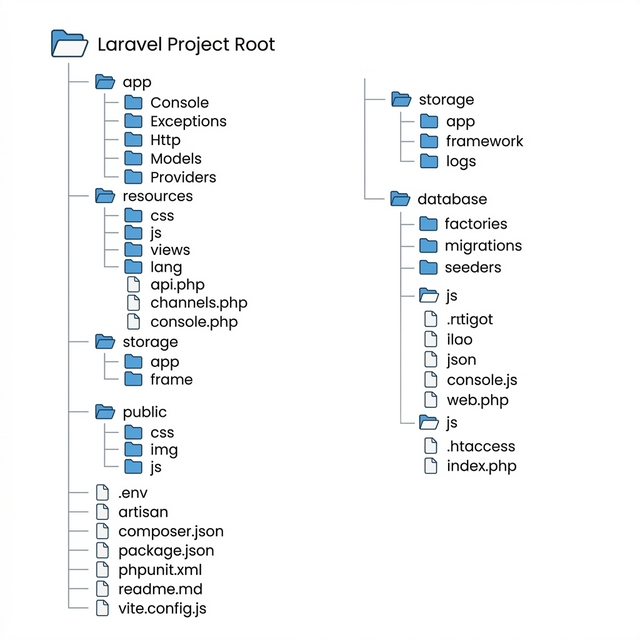
\includegraphics[width=0.7\textwidth]{images/folder_structure.png}
    \caption{Laravel Project Folder Hierarchy}
\end{figure}

\section{Local Development Setup}
CivicGuard is designed to be easily deployed on local environments using Laravel Herd or a custom PHP/PostgreSQL setup for rapid development and testing.

\subsection{Prerequisites}
\begin{itemize}
    \item PHP $\geq$ 8.2
    \item PostgreSQL $\geq$ 14.0
    \item Composer 2.x
    \item Node.js & NPM
\end{itemize}

\subsection{Installation Steps}
\begin{enumerate}
    \item \textbf{Clone the Repository:} Download the project files into the `htdocs` directory.
    \item \textbf{Dependency Management:} Run `composer install` to fetch PHP libraries and `npm install` for frontend assets.
    \item \textbf{Configuration:} Copy `.env.example` to `.env` and configure the database credentials (`DB_DATABASE=asset_reporting`).
    \item \textbf{Storage Link:} Run `php artisan storage:link` to make uploaded report images accessible to the web.
    \item \textbf{Database Migration:} Run `php artisan migrate --seed` to create tables and populate initial roles.
    \item \textbf{Build Assets:} Run `npm run build` to compile Tailwind CSS and JavaScript.
\end{enumerate}

\section{Cloud Deployment Strategy}
For production environments, CivicGuard is optimized for deployment on Linux-based VPS providers (e.g., DigitalOcean, AWS, or Heroku). The production setup involves:
\begin{itemize}
    \item \textbf{Web Server:} Nginx configured as a reverse proxy for the Laravel application.
    \item \textbf{SSL Termination:} Encrypting all civic data with Let's Encrypt certificates to ensure citizen privacy.
    \item \textbf{Task Scheduling:} Configuring Laravel's Task Scheduler (Cron) to handle asynchronous notification broadcasting.
    \item \textbf{Environment Security:} Ensuring that the \texttt{.env} file is isolated and that debugging modes are disabled to prevent technical disclosure.
\end{itemize}

\section{Environment Configuration (\texttt{.env})}
The heartbeat of the deployment is the environment file. It contains sensitive credentials that should never be shared:
\begin{itemize}
    \item \texttt{APP_ENV=production} (Disables debug errors and optimizes performance).
    \item \texttt{DB\_CONNECTION=pgsql} (Specifies PostgreSQL as the database driver).
    \item \texttt{DB\_PORT=5432} (Default PostgreSQL port).
    \item \texttt{DB\_DATABASE=asset\_reporting} (Defines the primary storage target for PostgreSQL).
    \item \texttt{FILESYSTEM_DISK=public} (Ensures report photos are accessible to citizens for tracking).
\end{itemize}

\begin{figure}[H]
    \centering
    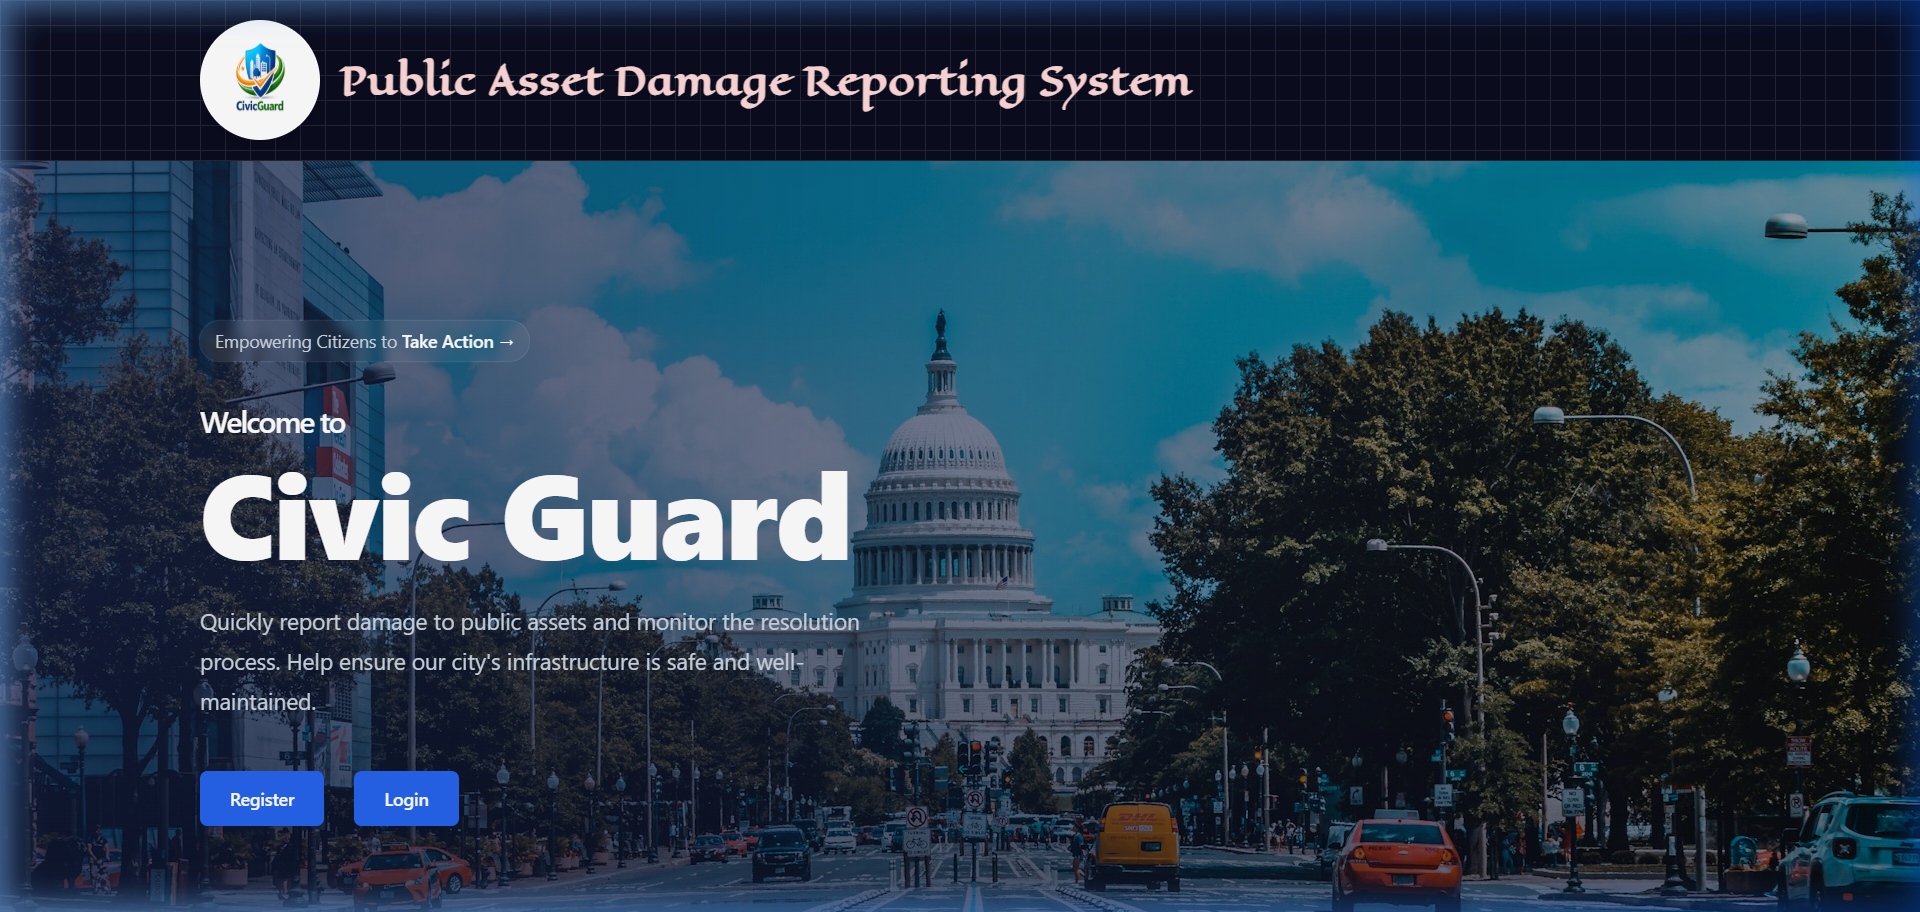
\includegraphics[width=0.85\textwidth]{images/landing_page.png}
    \caption{Project Hosting and Resource Management Strategy}
\end{figure}
